\documentclass[a4paper,11pt]{article}

\usepackage{mlsubmit}
\usepackage{bm}
\begin{document}

\initmlsubmision{3}                              					% assignment number
								{Raktim Mitra}      						           		% your name
								{150562}																		% your roll number

\begin{mlsolution}

\subsection*{Part 1:} We want to prove $\theta^{MLE}\epsilon$ arg $max_{\bm{\theta} \epsilon \Theta}$ $Q_{\bm{\theta}^{MLE}}(\bm{\theta}) $ with $\theta^{MLE} \epsilon$ arg $max_{\bm{\theta} \epsilon \Theta}$ $P[X | \bm{\Theta}] $.

\begin{center}
$Q_{\bm{\theta}^t}(\bm{\theta}) = \sum_{i=1}^{n}\mathbb{E}_{\vz\sim\mathbb{P}[\vz | \vx^i,\bm{\theta}^t]}log\mathbb{P}[\vx^i,\vz | \theta]$
\end{center} 
We can write: (by deviding with a term independent of $\bm{\theta}$)
\begin{center}
arg $max_{\bm{\theta} \epsilon \Theta}\sum_{i=1}^{n}\mathbb{E}_{\vz\sim\mathbb{P}[\vz | \vx^i,\bm{\theta}^t]}log\mathbb{P}[\vx^i,\vz | \theta] $\\[0.5em]
$= arg max_{\bm{\theta} \epsilon \Theta}\sum_{i=1}^{n}\mathbb{E}_{\vz\sim\mathbb{P}[\vz | \vx^i,\bm{\theta}^t]}log\frac{\mathbb{P}[\vx^i,\vz | \theta]}{\mathbb{P}[\vz | \vx^i,\bm{\theta}^t]}$
\end{center}
Now we can use two results derived in lecture 16: $$log P[X |\theta^{MLE}] = \sum_{i=1}^{n}\mathbb{E}_{\vz\sim\mathbb{P}[\vz | \vx^i,\bm{\theta}^{MLE}]}log\frac{\mathbb{P}[\vx^i,\vz | \theta^{MLE}]}{\mathbb{P}[\vz | \vx^i,\bm{\theta}^{MLE}]}$$ and $$log P[X |\theta] \geq \sum_{i=1}^{n}\mathbb{E}_{\vz\sim\mathbb{P}[\vz | \vx^i,\bm{\theta}^{MLE}]}log\frac{\mathbb{P}[\vx^i,\vz | \theta]}{\mathbb{P}[\vz | \vx^i,\bm{\theta}^{MLE}]}\quad \forall \theta$$ 
Since, $\theta^{MLE}$ maximises $log \mathbb{P}[\vx | \theta]$
$$log P[X |\theta^{MLE}] \geq \sum_{i=1}^{n}\mathbb{E}_{\vz\sim\mathbb{P}[\vz | \vx^i,\bm{\theta}^{MLE}]}log\frac{\mathbb{P}[\vx^i,\vz | \theta]}{\mathbb{P}[\vz | \vx^i,\bm{\theta}^{MLE}]}\quad \forall \theta$$ i.e.
$$log P[X |\theta^{MLE}] \geq Q_{\bm{\theta}^t}(\bm{\theta})$$ Therefore, $\theta^{MLE}$ maximises $\geq Q_{\bm{\theta}^t}(\bm{\theta})$ too. i.e.  $\theta^{MLE} \epsilon$ arg $max_{\bm{\theta} \epsilon \Theta}$ $P[X | \bm{\Theta}] $. [Proved]
%\begin{figure}[th]%
%\centering
%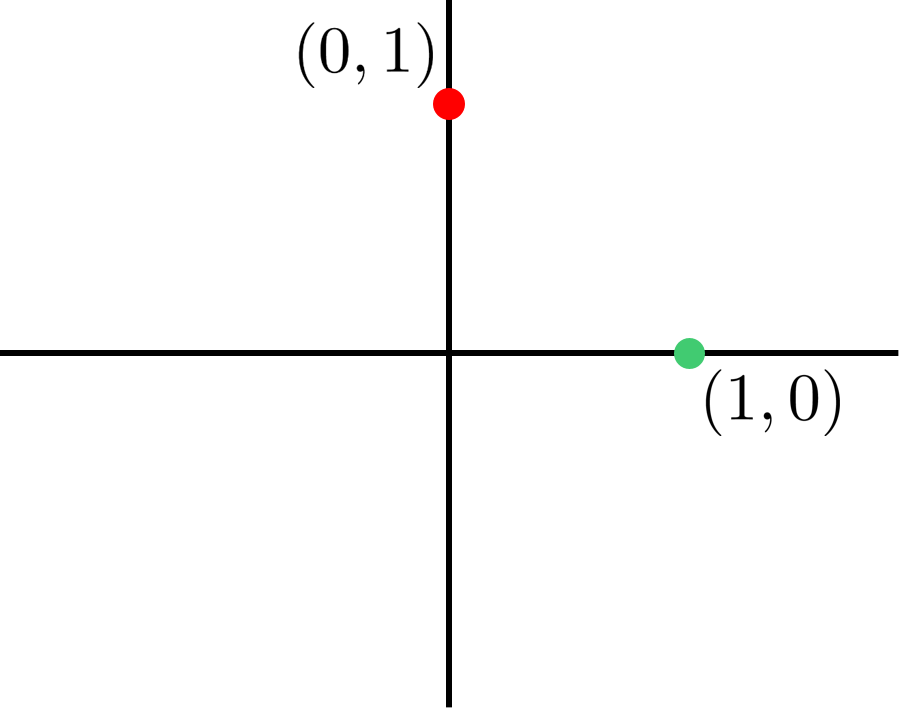
\includegraphics[width=0.3\columnwidth]{proto_blank.png}%
%\hfill
%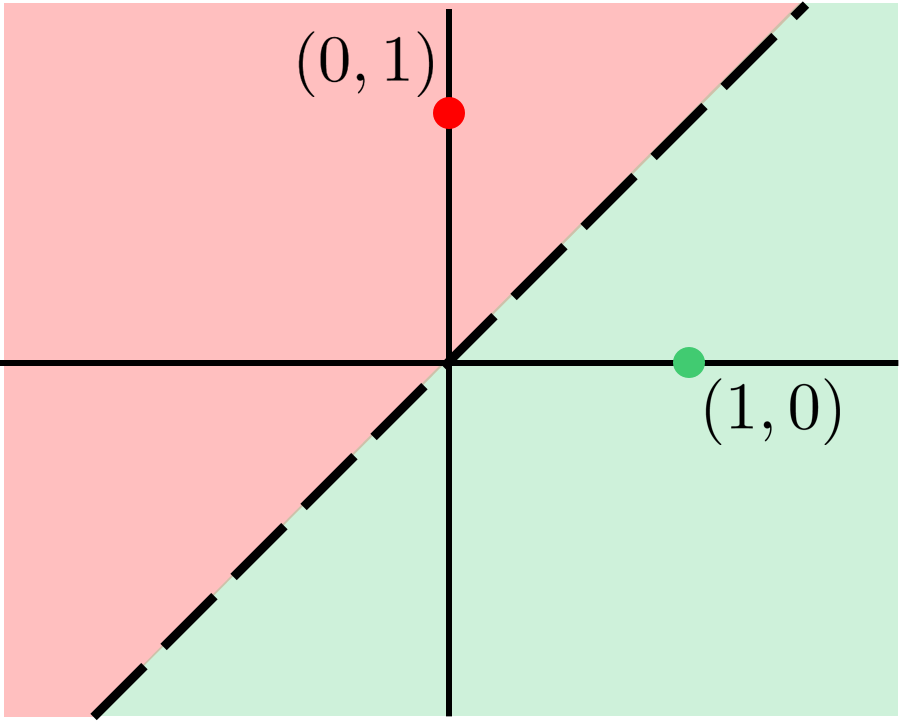
\includegraphics[width=0.3\columnwidth]{proto_euclid_sample.png}%
%\caption{Learning with Prototypes: the figure on the left shows the two prototypes. The figure on the right shows what the decision boundary if the distance measure used is $d(\vz^1,\vz^2) = \norm{\vz^1-\vz^2}_2$, for any two points $\vz^1,\vz^2 \in \bR^2$. The decision boundary in this case is the line $y = x$.}%
%\label{fig:proto}%
%\end{figure}

\end{mlsolution}
%------------------------q2--------------------------
\begin{mlsolution}
\subsection*{Part 1:}
For some partition $\{\Omega_i\}_{i=1,...,n}$ of $\mathbb{R}^d$ and weights $\{\vw^i\}_{i=1,..,n}$, $f:\mathbb{R}^d \rightarrow \mathbb{R}$ is such that $\forall \mathbf{x} \epsilon \mathbb{R}^d$
\begin{center}
$f(\vx) = \sum_{i=1}^{n}\mathbb{I}\{\vx \epsilon \Omega_i \}.\langle \vw^i,\vx\rangle$
\end{center}
The function $g(\vx) = c.f(\vx)$ can be written as:
\begin{center}
$g(\vx) = c\sum_{i=1}^{n}\mathbb{I}\{\vx \epsilon \Omega_i \}.\langle \vw^i,\vx\rangle$\\

$= \sum_{i=1}^{n}\mathbb{I}\{\vx \epsilon \Omega_i \}.\langle c\vw^i,\vx\rangle$
\end{center}
Thus for same partition $\{\Omega_i\}_{i=1,...,n}$ of $\mathbb{R}^d$ and weights $\{\vw'^i\}_{i=1,..,n}$, where $\vw'^i = c\vw^i$ $\forall i$\\
$\forall x\epsilon \mathbb{R}^d$ $g:\mathbb{R}^d \rightarrow \mathbb{R}$ can be written as :
\begin{center}
$g(\vx) = \sum_{i=1}^{n}\mathbb{I}\{\vx \epsilon \Omega_i \}.\langle \vw'^i,\vx\rangle$
\end{center}
which means $g(x)$ is piecewise lineaer. [Proved]

\subsection*{Part 2:}
Let, For some partition $\{\Omega_i^f\}_{i=1,...,n}$ of $\mathbb{R}^d$ and weights $\{\vw^i_f\}_{i=1,..,n}$, $f:\mathbb{R}^d \rightarrow \mathbb{R}$ is such that $\forall \mathbf{x} \epsilon \mathbb{R}^d$
\begin{center}
$f(\vx) = \sum_{i=1}^{n}\mathbb{I}\{\vx \epsilon \Omega_i^f \}.\langle \vw^i_f,\vx\rangle$
\end{center}
and Let, For some partition $\{\Omega_i^g\}_{i=1,...,n}$ of $\mathbb{R}^d$ and weights $\{\vw^i_g\}_{i=1,..,n}$, $f:\mathbb{R}^d \rightarrow \mathbb{R}$ is such that $\forall \mathbf{x} \epsilon \mathbb{R}^d$
\begin{center}
$g(\vx) = \sum_{i=1}^{n}\mathbb{I}\{\vx \epsilon \Omega_i^g \}.\langle \vw^i_g,\vx\rangle$
\end{center}
for $\vx$ $\epsilon$ $\mathbb{R}^d$ let, $h(\vx) = f(\vx) + g(\vx)$ the,, since $\vx$ can belong to only one of $\Omega_i^fs$ and one of $\Omega_i^gs$, we have to add only two terms. Say, $\vx \epsilon \Omega_k^f$ and $\vx \epsilon \Omega_l^g$ with weights $w^k_f,w^l_g $ repectively.
\begin{center}
hence, $h(\vx) = \langle w^k_f,\vx\rangle + \langle w^l_g,\vx\rangle $\\

$=\langle w^k_f+w^l_g,x \rangle$
\end{center}
Now we construct a new partition $\Omega^h$ for $h(\vx)$ using above observation:\\
For each partition $\Omega_i^f$ let, $S_i$ be the set of $\Omega_j^gs$ such that $\Omega_i^f \cap \Omega_j^g \neq \phi$. For each element $\Omega_j^g$ of $S_i$ add set $\Omega_i^f \cap \Omega_j^g $ as $\Omega_{ij}^h$ to $\Omega^h$. 

By the construction and by the disjointeness of each partition subsets, $\vx$ $\epsilon$ $\Omega_{ij}^h \leftrightarrow$ $\vx$ $\epsilon$ $\Omega_{i}^f \& $  $\vx$ $\epsilon$ $\Omega_{j}^g$. hence we can define new weights $\vw_h^{ij} = \vw_f^i + \vw_g^j$ for all $\Omega^h_{ij} \epsilon \Omega^h$.

Hence, for partition $\Omega^h$ , weights $\{\vw_h^{ij}\}s$ for $\vx \epsilon \mathbb{R}^d$, $h(\vx):\mathbb{R}^d \rightarrow \mathbb{R}$
\begin{center}
$h(\vx) = \sum_{\Omega_{ij}^h\epsilon\Omega^h}\mathbb{I}\{\vx \epsilon \Omega_{ij}^h \}.\langle \vw^{ij}_h,\vx\rangle$
\end{center}
Hence. $h(\vx)$ is piecewise linear. [Proved] 
\newpage
\subsection*{Part 3:}
Let, For some partition $\{\Omega_i\}_{i=1,...,n}$ of $\mathbb{R}^d$ and weights $\{\vw^i\}_{i=1,..,n}$, $f:\mathbb{R}^d \rightarrow \mathbb{R}$ is such that $\forall \mathbf{x} \epsilon \mathbb{R}^d$
\begin{center}
$f(\vx) = \sum_{i=1}^{n}\mathbb{I}\{\vx \epsilon \Omega_i \}.\langle \vw^i,\vx\rangle$
\end{center}
now, $g(\vx) = f_{ReLU}(f(\vx)) = max(f(\vx),0)$, then for some $\vx \epsilon \mathbb{R}^d$:
\begin{center}
$g(\vx) = \sum_{i=1}^{n}\mathbb{I}\{\vx \epsilon \Omega_i \}.max(\langle \vw^i,\vx\rangle,0)$\\

$= \langle \vw^k,\vx\rangle when \langle \vw^k,\vx\rangle > 0$ $and $ $= 0$ when $\langle \vw^k,\vx\rangle \leq 0 $, $x \epsilon \Omega_k$
\end{center} 

From above observation we can say that by applying ReLU we are basically passing a plane $\langle \vw^k,\vx\rangle = 0$ through $\Omega_k$ and assiging 0 to $h(\vx)$ for $\vx$ lying on $\leq 0 $ side of the plane. In other words we can make $w^k$ = 0 in those regions.

Therefore we create a new partition $\Omega'$ with $2n$ subsets $\{\Omega_{i1},\Omega_{i2}\}_{i=1,...,n}$ where $\Omega_{i1}$ corresponds to set of $\vx$'s such that  $\langle \vw^i,\vx\rangle > 0$ and we define $\vw'^{i1} = \vw^i$, $\Omega_{i2}$ corresponds to set of $\vx$'s such that  $\langle \vw^i,\vx\rangle \leq 0$ and we define $\vw'^{i2} = 0$.
Then, we represent these new weights as $\{\vw'^i\}_{i=1,2,...,2n}$. i.e. $\vw^{jk} =\vw'^{j*k} $. and also partition $\Omega'$ as $\{\Omega'_i\}_{i=1,2,...,2n}$. i.e. $\Omega_{jk} =\Omega'_{j*k} $

Now, for partition $\Omega'$ and weights $\{w'^i\}s$ $g(\vx): \mathbb{R}^d \rightarrow \mathbb{R}$ can be represented as:
\begin{center}
$g(\vx) = \sum_{i=1}^{2n}\mathbb{I}\{\vx \epsilon \Omega'_i \}.\langle \vw'^i,\vx\rangle$\\
\end{center}
Hence, $g(x) = f_{ReLU}(f(\vx))$ is piecewise linear. [Proved]

\subsection*{Part 4:}
\textbf{Claim:} Any neural network with a ReLU activation function computes a piecewise linear function.\\
\textbf{Proof by Induction:} 

\textbf{\textit{Hypothesis}}

In a network with only ReLU activation function, if all neuron's in $i^{th}$ layer outputs a piecewise linear activation function then so does $i+1^{th}$ layer of the network.\\
\textbf{\textit{Base Case}}

The input nodes may or may not have ReLU activation. 

If, input nodes do not have ReLU activation then we have linear functions being output from each of them (they basically output $\vx_i$ each) i.e. they are piecewise linear too. 

Else, they output $f_{ReLU}$ on a linear function which is again piecewise linear by part 3.\\
\textbf{\textit{Induction Step}}

Each neuron in $i+1^{th}$ layer ouputs $f_{ReLU}()$ applied on weighted sum of activation outputs of neuron's in previous layer it is connected to.

let, a neuron in $i+1^{th}$ layer is connected to m neuron's in $i^{th}$ layer. Let, activation outputs by them are $\{f_i\}_{i=1,...,m}$ and each connection edge has $\{\vw^i\}_{i=1,...,m}$. The neuron in $i+1^{th}$ layer therefore outputs $f_{ReLU}(\sum_{i=1}^{m}w^i.f_i)$

Now, since each $f_i$ is piecewise linear, then by part 1 of the problem, so is $w^i.f_i$.(constant multiplication)

Now, by part 2 of the problem,  $\sum_{i=1}^{m}w^i.f_i$ is also piecewise linear (sum of piecewise linear functions)

Now, by part 3 of problem, $f_{ReLU}(\sum_{i=1}^{m}w^i.f_i)$ is piecewise linear, since $\sum_{i=1}^{m}w^i.f_i$ is piecewise linear. 

Therefore the neuron in $i+1^{th}$ layer outputs piecewise linear function. This applies for all neurons in $i+1^{th}$ layer.

Hence, by induction the claim holds. [Proved]

\subsection*{Part 5:}
\begin{itemize}
\item The network has d input nodes, D hidden layer nodes on a single hidden layer with ReLU activation and one output node with ReLU activation.
\item Each  hidden layer node gets a input $\epsilon$ $\mathbb{R}^d$. It outputs a piecewise linear function  with 2 pieces(uses one ReLU on a linear function). So, basically each hidden node outputs a function which has two pieces basically signifying a hyperplane on $\mathbb{R}^d$.

\item The piecewise linear function that is sent to output node as input is weighted sum of outputs by the hidden nodes. Weight multiplication does not change partition. The sum however, changes the partition and total number of partition now can be upper bounded by maximum number of regions D (d-1) dimensional hyperplanes can create in a d dimensional space. Let $L^{D}_{d}$ be the number of regions. This is given by the recursion $$L^{D}_{d} = L^{D-1}_{d} + L^{D-1}_{d-1}$$ We can solve it to get $$L_{d}^{D} = \sum_{i=0}^{d}{D\choose i}$$.
Therefore input to output node is a piecewise linear function with at most $L_{d}^{D}$ pieces. 
\item The output node applies another ReLU on it. Which may at max devide each piece into 2 pieces. Therefore, maximum number of pieces possible becomes $$2L_{d}^{D} = 2\sum_{i=0}^{d}{D\choose i}$$
\end{itemize}
\end{mlsolution}
%------------------------q3--------------------------
\begin{mlsolution}
\begin{mlalgorithm}[0.9\textwidth]{h!}{Kernel Perceptron: }\vskip-2ex
	\label{algo:tk-means}
	\begin{algorithmic}[1]
		\REQUIRE Receive a data point $(x^t,y^t)$ $\epsilon$ $\chi $ at each timestamp.
		\STATE Initialize $\mathbf{\alpha}$ with 0 length vector. //$\mathbf{\alpha}$ will be of size t at timestamp t
		\STATE We store older $(\vx^i,y^i)$s to calculate update for incoming points.
		\WHILE{data points are incoming }
			\STATE{At each timestep t:}
			\STATE receive $(\mathbf{x}^t,y^t)$ and increase size of $\mathbf{\alpha}$ by adding another 0 coordinate.
				\STATE ${\displaystyle {\hat {y}}=\operatorname {sgn} \sum _{j=1}^{t}\alpha _{j}y_{j}K(\mathbf {x} ^{j},\mathbf {x} ^{t})}$
				\IF {$\hat{y} \neq y_i$} 
				\STATE$\alpha_i \leftarrow \alpha_i + 1$
				\ENDIF
		\ENDWHILE
		\STATE  predict $y_{test}$ for a testpoint $x_{test}$ by, ${\displaystyle {\hat {y}}=\operatorname {sgn} \sum _{j=1}^{t}\alpha _{j}y_{j}K(\mathbf {x} ^{t},\mathbf {x} ^{j})}$\\\hfill //from dual version of the perceptron
	\end{algorithmic}
\end{mlalgorithm}
\end{mlsolution}
%------------------------q4--------------------------
\begin{mlsolution}
\subsection*{Part 1:}
$K(\vz^1,\vz^2) = (\langle\vz^1,\vz^2\rangle + 1)^2 = (x_1x_2 + y_1y_2 + 1)^2 = x_1^2x_2^2 + y_1^2y_2^2 + 2x_1x_2y_1y_2 + 2x_1x_2 + 2y_1y_2 + 1$\\

We want to represent $K(\vz^1,\vz^2) = \langle\phi(\vz^1),\phi(\vz^2)\rangle $ we take $\mathcal{H}_K \equiv{\mathbb{R}^6}$ because $K(\vz^1,\vz^2) $ has 6 terms, to represent it as a scalar product, we need vectors with 6 dimensions.

Thus our construction follows from the expression :

\begin{center}
$\phi(\vz)=\phi(x,y)=[x_1^2,y_1^2,\sqrt{2}xy,\sqrt{2}x,\sqrt{2}y,1]$ 
\end{center}
Clearly,  $K(\vz^1,\vz^2) = \langle\phi(\vz^1),\phi(\vz^2)\rangle $. Hence K is Mercer. [Proved]
\subsection*{Part 2:}
For given $f_{(A,\vb,c)} = \langle\vz,A\vz\rangle + \langle\vb,\vz\rangle + c$ where \[
   A=
  \left[ {\begin{array}{cc}
   a_{11} & a_{12} \\
   a_{21} & a_{22} \\
  \end{array} } \right]
\]and \[\vb =  \left[ {\begin{array}{cc}
   b_1 & b_2 \\
  \end{array} } \right]^T
  \]
  Then, $f_{(A,\vb,c)} = a_{11}x^2 + (a_{21} + a_{12})xy + a_{22}y^2 + b_1x + b_2y + c$
  
  Let, $\vw=[w_1,w_2,w_3,w_4,w_5,w_6]^T$, then: $$\langle\vw,\phi(\vz)\rangle = w_1x^2 + w_2y^2 + \sqrt{2}w_3xy +\sqrt{2} w_4x +\sqrt{2} w_5y + w_6$$ 
  comparing $f_{(A,\vb,c)} = \langle\vw,\phi(\vz)\rangle$ \\
  we have $w_1 = a_{11},w_2 = a_{22},w_3 = \frac{a_{21} + a_{12}}{\sqrt{2}}, w_4 = \frac{b_1}{\sqrt{2}},w_5 = \frac{b_2}{\sqrt{2}},w_6 = c$\\
  
  Therefore, required $\vw$ is $[a_{11},a_{22},\frac{a_{21} + a_{12}}{\sqrt{2}},\frac{b_1}{\sqrt{2}},\frac{b_2}{\sqrt{2}},c]^T$[Answer]

\subsection*{Part 3:}

For given $\vw = [w_1,w_2,w_3,w_4,w_5,w_6]^T$, we know:
$$\langle\vw,\phi(\vz)\rangle = w_1x^2 + w_2y^2 + \sqrt{2}w_3xy +\sqrt{2} w_4x +\sqrt{2} w_5y + w_6$$

We want to construct $(A,\vb,c)$ $\epsilon$ $\mathbb{R}^{2\times 2}\times\mathbb{R}^2\times\mathbb{R}$ where, \[
   A=
  \left[ {\begin{array}{cc}
   a_{11} & a_{12} \\
   a_{21} & a_{22} \\
  \end{array} } \right]
\]and \[\vb =  \left[ {\begin{array}{cc}
   b_1 & b_2 \\
  \end{array} } \right]^T
  \]
  and $f_{(A,\vb,c)} = a_{11}x^2 + (a_{21} + a_{12})xy + a_{22}y^2 + b_1x + b_2y + c$\\  
  
  again comparing $f_{(A,\vb,c)} = \langle\vw,\phi(\vz)\rangle$ \\
  we have = $a_{11} = w_{1},a_{22} = w_{2}, b_1 = \sqrt{2}w_4,b_2 = \sqrt{2}w_5,c = w_6$, aand as can be seen $w_3 = \frac{a_{21} + a_{12}}{\sqrt{2}}$, therefore $a_{21},a_{12}$ can have infinitely possible values such that the relation with $w_3$ holds. To make things symmetrical we can take $a_{21} = a_{12} = \frac{\sqrt{2}w_3}{2} = \frac{w_3}{\sqrt{2}}$ \\
  
  Hence required construction :\[
   A=
  \left[ {\begin{array}{cc}
   w_{1} & \frac{w_3}{\sqrt{2}} \\
   \frac{w_3}{\sqrt{2}} & w_{2} \\
  \end{array} } \right]
\]and \[\vb =  \left[ {\begin{array}{cc}
   \sqrt{2}w_4 & \sqrt{2}w_5 \\
  \end{array} } \right]^T
  \]
  and $$c = w_6$$
 
\subsection*{Part 4:}
\begin{itemize}
\item Let, $f_{A,b,c}$ minimises least square error on the right hand side. By, part 2 of the problem it can be converted to $\langle w_r,\phi(x)$.
\item The solution for Kernel Ridge regression with regularization $\lambda$ let the corresponding weight be $w_l$. By part 3, $w_l$ corresponds to a quadratic function too.  Let, $L_l$ denote the total error on left side(kernel ridge side).
\end{itemize}

%Now, let $|| w_i - w_r || = \delta$ and $|| L_i - L_r || \leq p\delta^2 + q\delta $ for some $w_i$.

We can see : $$|| L_i - L_r || = \sum_{j=1}^{n}(y^j - \langle w_i,\phi(\vz^j)\rangle)^2 - (y^j - \langle w_r,\phi(\vz^j)\rangle)^2$$ $$ = \sum_{j=1}^{n}(2y^j - \langle w_i + w_r,\phi(z^j)\rangle)(\langle w_r - w_i,\phi(z)^j \rangle)$$ 
$$\leq ||w_i - w_r||\sum_{i=1}^{n}(2y^j - \langle w_i + w_r,\phi(z^j)\rangle)||\phi(z^j)||$$

Let, $X \epsilon \mathbb{R}^{n \times 6}$ and $y \epsilon \mathbb{R}^n$ contains our $\phi$ mapped input vectors.  

We have known results for $w_l$ and $w_r$ : $$w_r = (X^{T}X)^{-1}X^Ty$$ and $$w_l = (X^TX + \lambda I)^{-1}X^Ty$$

We can do this because $\phi$ is not very high dimensional.\\
$X^TX$ is a psd matrix and can be written as $UAU^T$ where A is diagonal matrix with  $\geq$ entries $(a1,a_2,...)$. then we have \\
\begin{center}
$w_l - w_m = U(diag(1/a_i - 1/(a_i + \lambda))U^TX^Ty$ \\
$\leq \lambda U(diag(1/a_i^2))U^T X^Ty$\\ i.e. $||w_l - w_m|| \rightarrow 0 as \lambda \rightarrow 0$ i.e. Diffrence between two losses tends to 0. [Proved]
\end{center}
\end{mlsolution}
%------------------------q5--------------------------	
\begin{mlsolution}
$P[\vX \cond \vmu, \vW, \sigma ] = \mathcal{N}(\vx \cond \vmu, \vC)$ where	$\vC = \vW\vW^T + \sigma^2I_d$
	The data log-likelihood is given as:
	\begin{align*}
		L(\vTheta) &= log\ \prod_{i=1}^{n}P(\vX^i \cond \vmu, \vW, \sigma)	\\
					&= \sum_{i=1}^{n} log\ P(\vX^i \cond \vmu, \vW, \sigma)\\ 
					&= \sum_{i=1}^{n} log \frac{1}{(2\pi)^{\frac{d}{2}}|\vC|^\frac{1}{2}}
					exp({\frac{(\vX^i - \vmu)^T\vC^{-1}(\vX^i - \vmu)}{2}})\\
					&= \sum_{i=1}^{n} -\frac{d}{2}log2\pi - \frac{1}{2}|\vC| - \frac{(\vX^i - \vmu)^T\vC^{-1}(\vX^i - \vmu)}{2}\\
					&= -\frac{nd}{2}log2\pi - \frac{n}{2}|\vC| - \sum_{i=1}^{n}\frac{(\vX^i - \vmu)^T\vC^{-1}(\vX^i - \vmu)}{2}
					\intertext{Differentiating w.r.t $\vmu$ suing $\frac{\partial \vx^T \vA \vx}{\partial \vx} = \vx^T\vA + \vx^T\vA^T$}
					0 &= \sum_{i=1}^{n} (\vX^i - \vmu)^T(\vC^{-1} + (\vC^{-1})^T)\\
					\implies 0 &= (\vC^{-1} + (\vC^{-1})^T) \sum_{i=1}^{n} (\vX^i)^T- n\vmu^T\\
					\intertext{multiplying by $((\vC^{-1} + (\vC^{-1})^T))^{-1}$ since $\vC$ is invertible}\\
					\implies \vmu^T& = \frac{\sum_{i=1}^{n} (\vX^i)^T}{n}\\
					\implies \vmu& = \frac{\sum_{i=1}^{n} \vX^i}{n}
	\end{align*}
	
	i.e. MLE estimate for $\vmu$ is $\vmu^{MLE} = \frac{\sum_{i=1}^{n} \vX^i}{n}$
\end{mlsolution}				
\end{document}








































